\documentclass[../main.text]{subfiles}
\begin{document}
\section{Densities from Distributions}



Many multivariate visualizations treat the data space as a graph where the vertices's are the variables and the edge corresponds to some quantified relationship between the two vertexes and often these edges are colored by category or form a shape that can be used a proxy for a category. These types of visualizations can often be used to derive typical observations in a given category.


\begin{figure}
  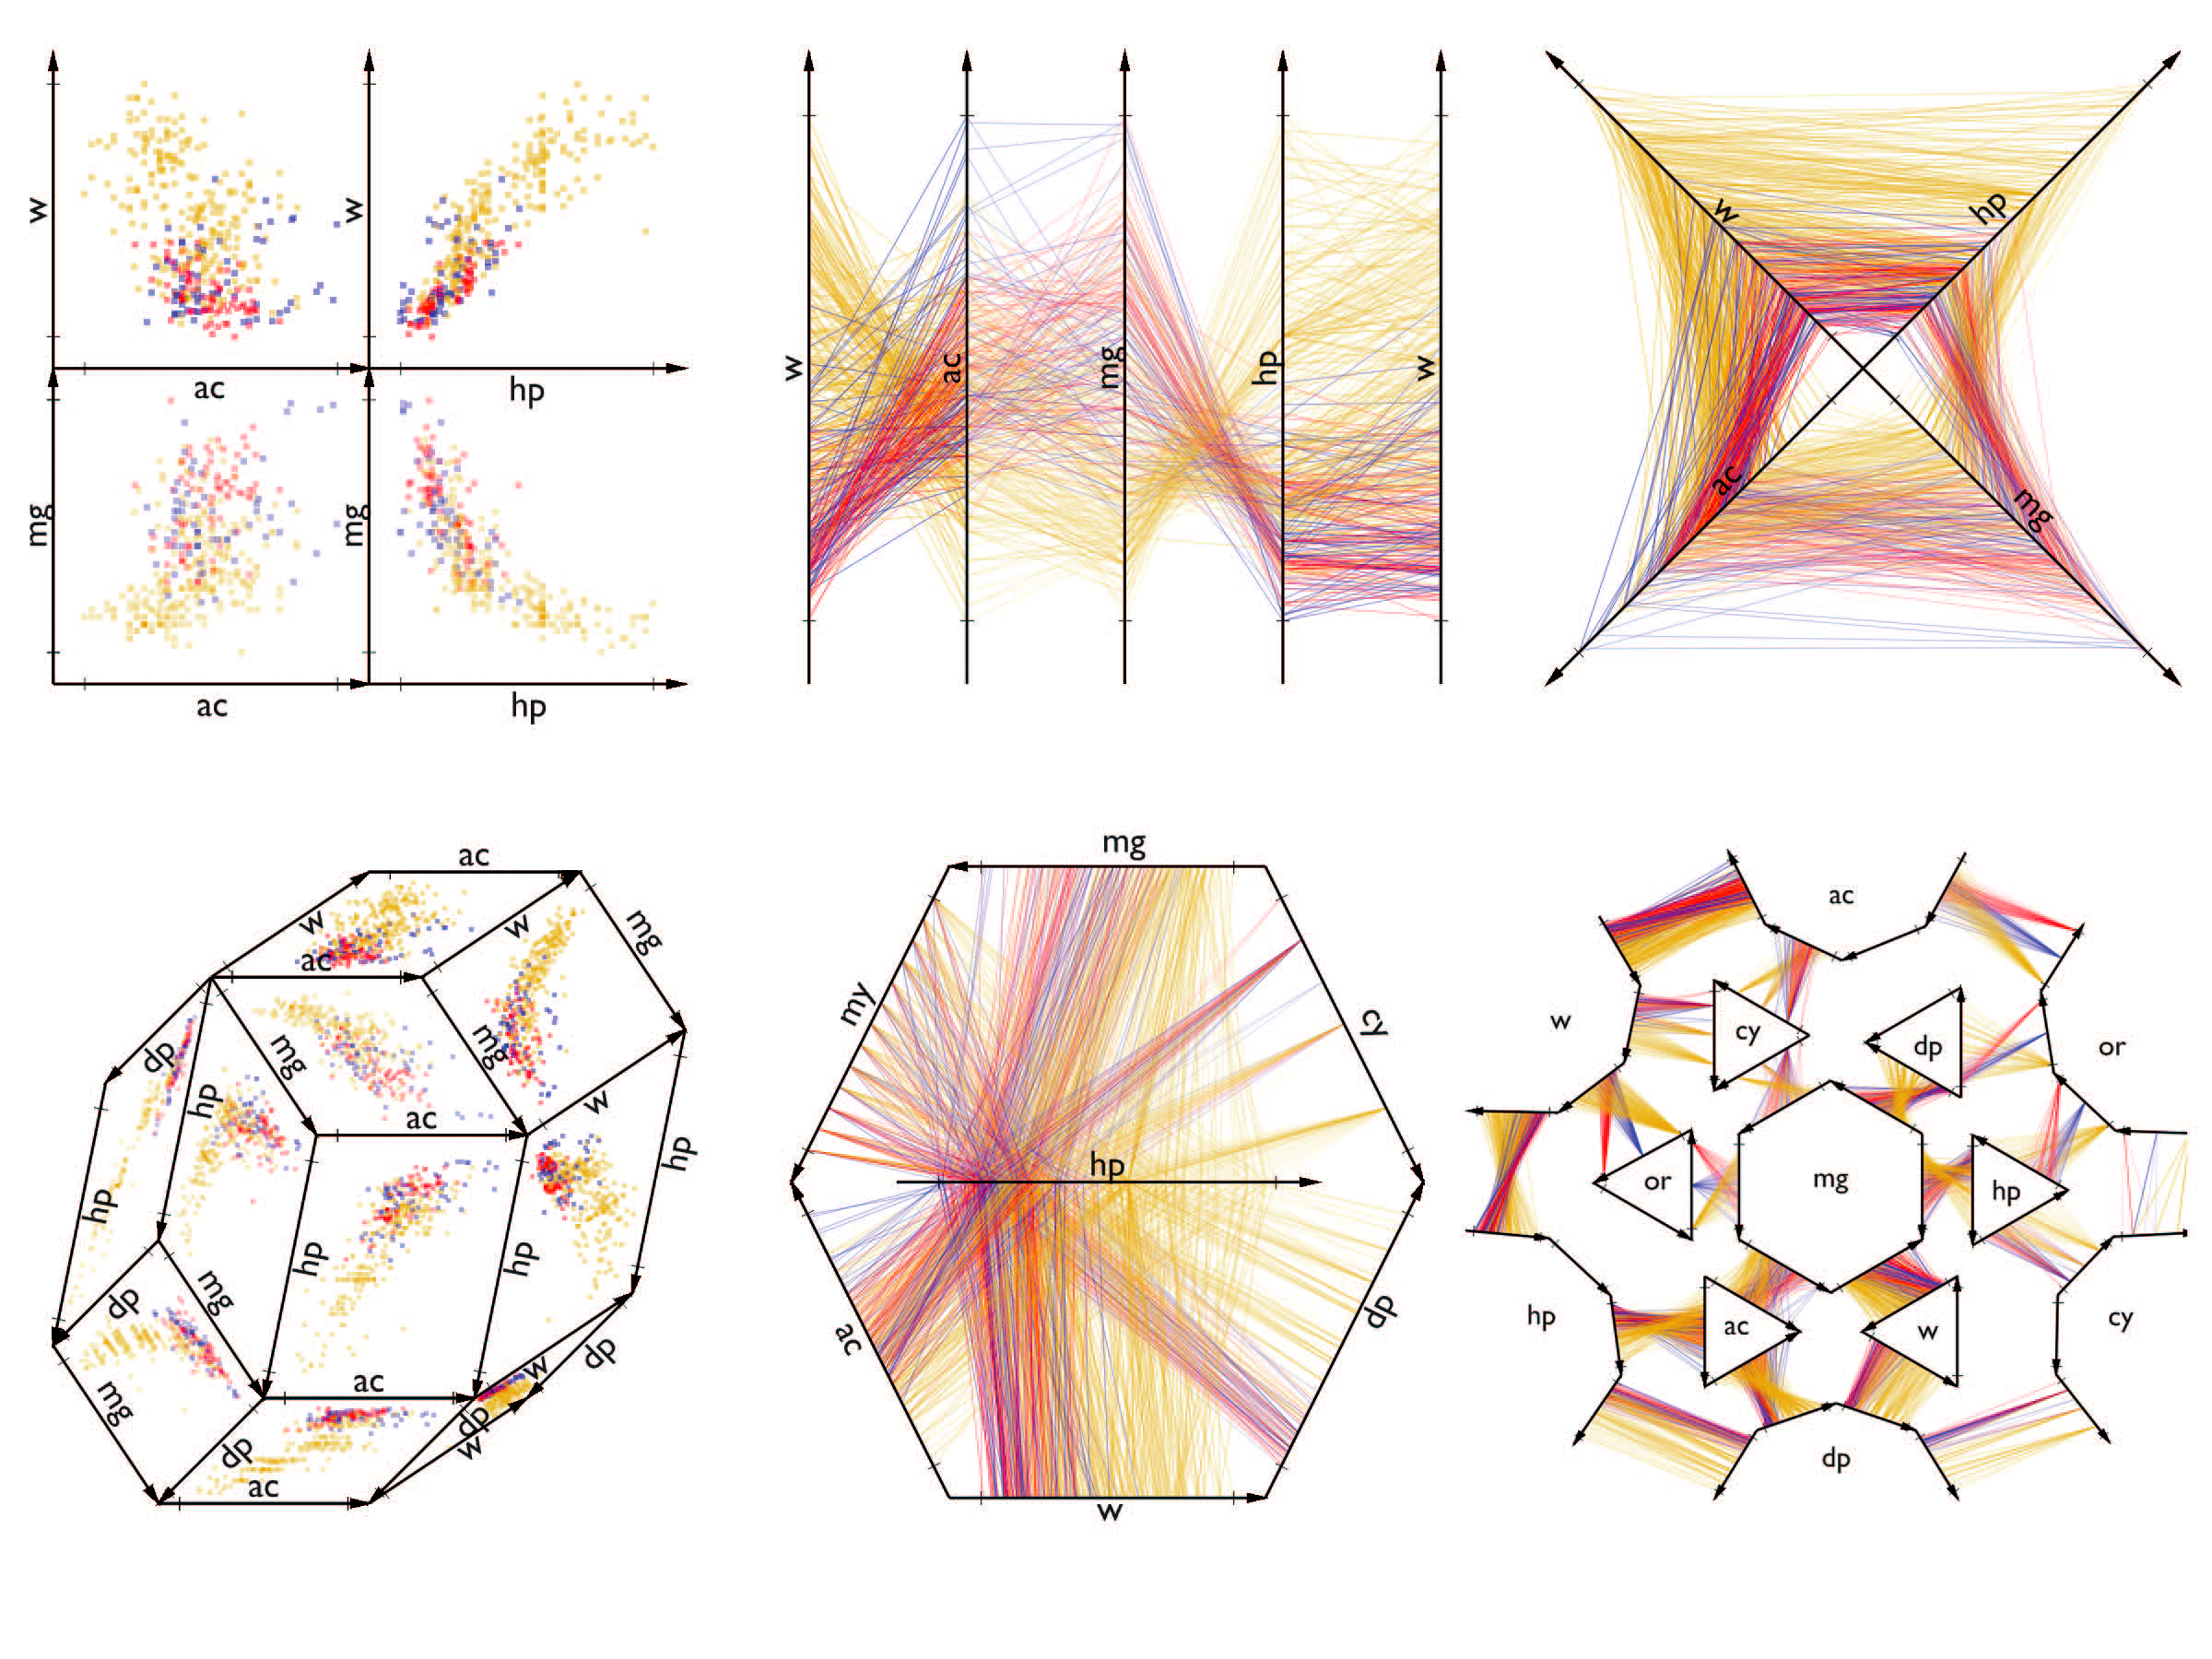
\includegraphics{flexaxis.png}
  \caption{Figure taken from \cite{claessen_flexible_2011} illustrates the following common
    methods for visualizing multivariate datasets: matrix of scatters, parallel coordinates and radar charts.
  \label{fig:flexlink}
\end{figure}

There are a number of methods for showing how measurements of different
variables interact, and as showing figure~\ref{fig:flexlink} color is often
used to illustrate how these relationships are different for each category of
data. As seen in figure~\ref{fig:flexlink}, the common methods for showing
visualizations are matrix of scatters \cite{elmqvist_rolling_2008} , parallel
coordinates \cite{inselberg_plane_1985, wegman_hyperdimensional_1990} and radar charts\cite{chambers_graphical_1983}.

\begin{figure}
  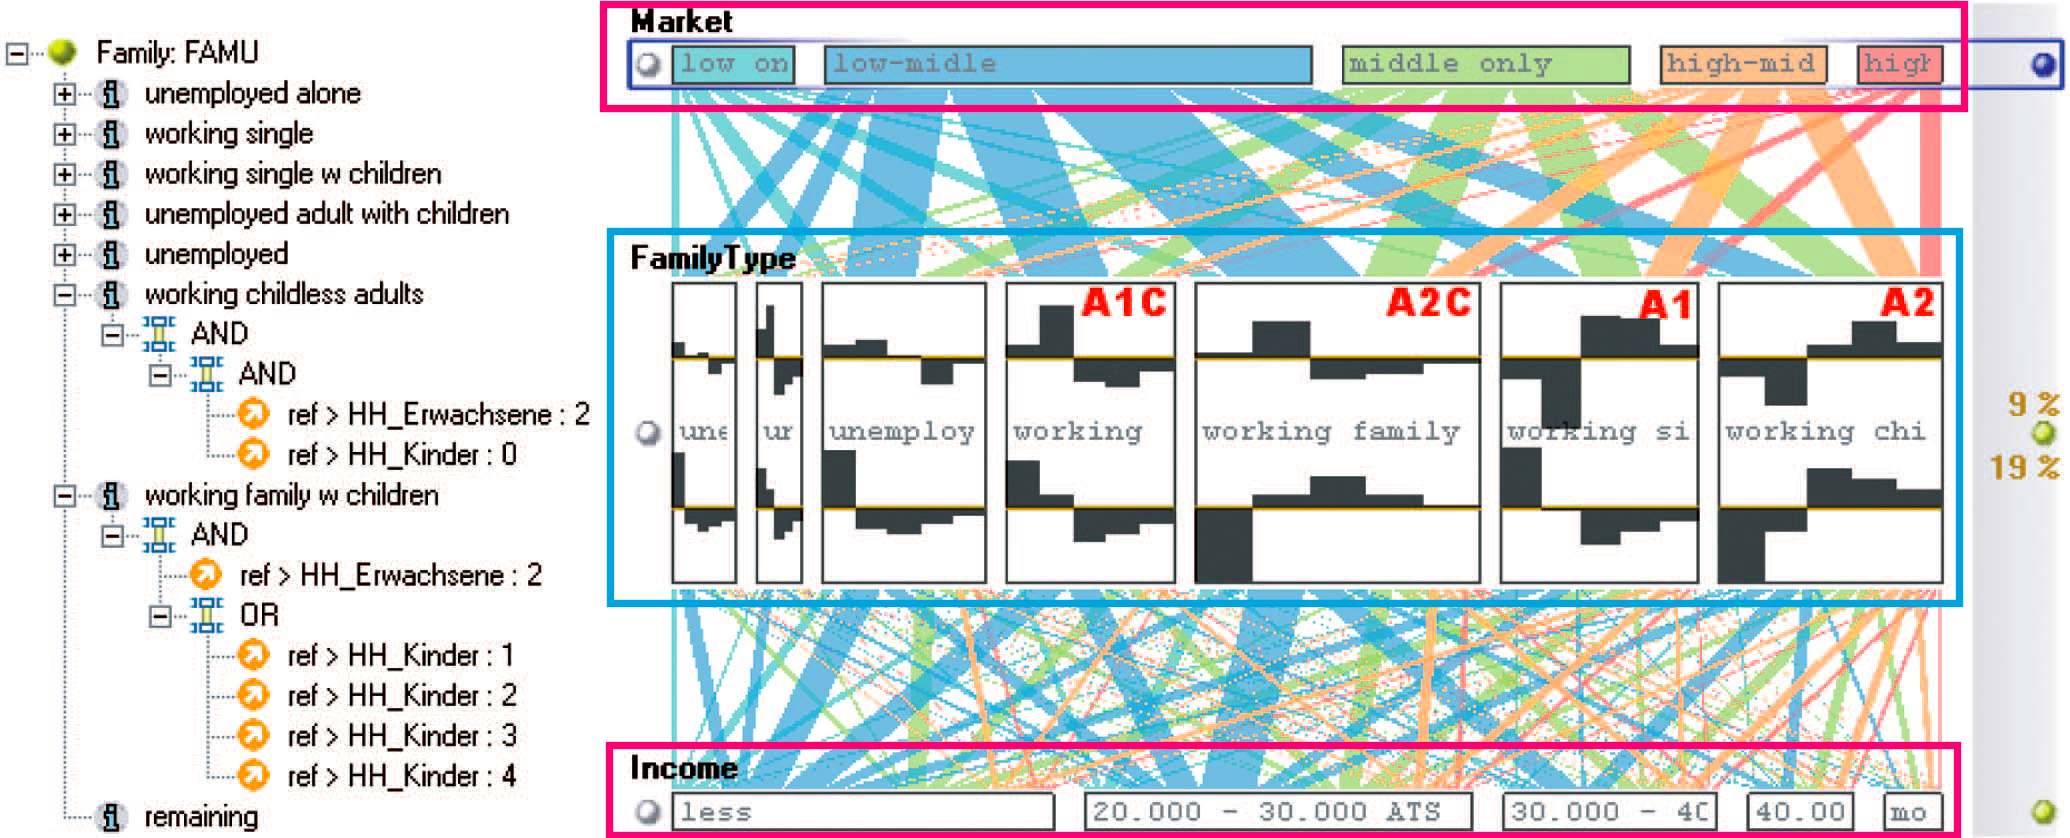
\includegraphics{parallelsets.png}
  \caption{On the left is the categorical view, where users can define
    categories based on other categorical information. For example, in this
    view working family with children is defined as a household with one or
    more children. On the right is a parallel coordinate graph where the
    dominant category informs the colors, the size of the box is relative to
    the category size, and the histograms show the frequencies of those
    categories relative to the connecting categories (market type and income
    respectively)}
  \label{fig:parallelsets}
\end{figure}

Another important factor in visualizing categorical data is retaining the
inherent hierarchy in many datasets with categorical measurements
\cite{shneiderman_visualizing_2000}. The Parallel Sets tool
showin in figure~\ref{fig:parallelsets} is explicitly designed to show frequencies
of set membership in heirarichal ordered categorical sets \cite{kosara_parallel_2006}. Building on the flexible linked axis version of
  the parallel coordinates plot \cite{claessen_flexible_2011}, Parallel Sets
  treats each categorical set independently but indicates conditional
  dependency through cross tabulations and by grouping the data, indicated via
  color, based on an active dimension that then becomes the pivot point for the
  cross tabulations. In Parallel Sets, quantitative data is converted to
  categorical via binning. Many-to-many PCP is another type of generalized
  parallel coordinates where all possible pairs are explored \cite{lind_many--many_2009}. 

\begin{figure}
  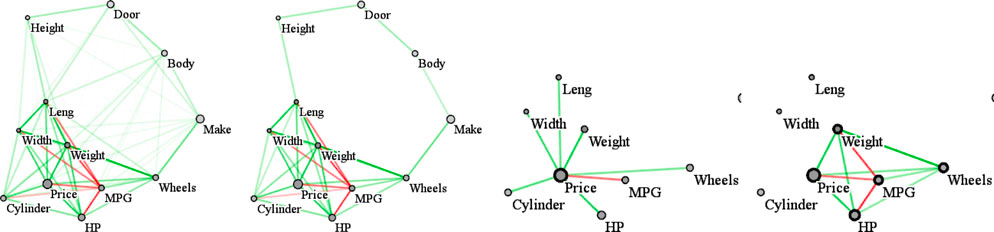
\includegraphics{corr.png}
  \label{caption} Zhang et al create an initial map (a) that they then apply an
  edge filter to (b). They then allow the user to filter out a variable and
  either highlight only the vertexes of that variable (c) or the edges incident
  on that variable(d).
  \label{fig:corr}
\end{figure}

Often though it's important to retain the internal structure of the
quantitative data, such as when the data is a function of time and
space. Zhang et al propose a method that retains data and allows for
visualizing more than just pairwise relationships\cite{zhang_visual_2015}. They
introduce a concept of a correlation map, as shown in
figure~\ref{fig:corr}. The authors build out a graph where every variable is a
vertex and the edges are correlations between the connecting vertexes. The
vertexes are sized relative to the variance in the data. The edges are colored
red for negative correlations and green for positive correlations. To convert
the categorical data to numerical space, they developed an algorithm where when
mapped to numbers, the residual sum of squares of a logistic regression of the
categorical variables  would be minimized. They then filter edges with low
correlations and on variables of interest.
\end{document}